%& -shell-escape -enable-write18 
\documentclass[uplatex,dvipdfmx]{jsarticle}
\usepackage[utf8]{inputenc}

\usepackage[dvipdfmx]{graphicx}
\usepackage[dvipdfmx]{color}
\usepackage[driver=dvipdfm,hmargin=19.05truemm,vmargin=25.40truemm]{geometry}
\usepackage{colortbl}
\usepackage{tcolorbox}
\usepackage{varwidth}
\usepackage{xcolor}
\PassOptionsToPackage{dvipsnames}{xcolor}

\usepackage{amsmath,amsfonts,amssymb,amsthm}
\usepackage{bm}
\usepackage[italicdiff]{physics}
\usepackage{mathtools}
\mathtoolsset{showonlyrefs=true}
\usepackage[unicode, dvipdfmx]{hyperref}
\usepackage{pxjahyper}
\hypersetup{
setpagesize=false,
    bookmarksnumbered=true,
    bookmarksopen=true,
    colorlinks=true,
    linkcolor=cyan,
    citecolor=red,
}
\usepackage{mathrsfs}
\usepackage{bussproofs}
\usepackage{enumerate}
\usepackage{pxrubrica}
\usepackage{tipa}
\usepackage{ascmac}
\usepackage{caption}
\usepackage[subrefformat=parens]{subcaption}
\usepackage{listings,jvlisting}
\usepackage{tikz}
\usetikzlibrary{math,patterns,intersections,calc,arrows,graphs}
\usepackage{float}
\usepackage{xparse}
\usepackage{url}
\usepackage{fancyhdr}
\usepackage{multicol}
\usepackage{siunitx}
\usepackage{hhline}
\usepackage{bxbase}
\usepackage[mark=***]{sectionbreak}
\usepackage[geometry]{ifsym}
\usepackage[prefernoncjk]{pxcjkcat}
\usepackage[LGR,T2A,T3,T1]{fontenc}
\usepackage[greek,latin,english,russian,japanese]{pxbabel}

\allowdisplaybreaks


\theoremstyle{definition}
\newtheorem{theorem}{Thm}
\newtheorem{corollary}{Col}
\newtheorem{lemma}{Lem}
\newtheorem{definition}{Def}
\newtheorem{proposition}{Prop}

\tcbuselibrary{most}

\renewcommand{\labelitemi}{$\circ$}
\renewcommand{\labelitemii}{$\triangleright$}

\ProvideDocumentCommand\floor{m}{\lfloor {#1} \rfloor}
\ProvideDocumentCommand{\where}{}{\mathrel{}\middle|\mathrel{}}
\ProvideDocumentCommand{\when}{m}{\quad({#1})}
\ProvideDocumentCommand{\adjoint}{}{\mathbf{\ast}}
\ProvideDocumentCommand{\conjugation}{}{\mathbf{\ast}}
\NewDocumentCommand{\Jacobi}{m m}{\frac{\partial ({#1})}{\partial ({#2})}}
\NewDocumentCommand{\JacobiPolar}{O{x,y}}{\frac{\partial ({#1})}{\partial (r,\theta)}}
\DeclareMathOperator{\Ker}{Ker}
\DeclareMathOperator{\Img}{Im}
\DeclareMathOperator{\res}{Res}
\DeclareMathOperator{\Dom}{Dom}
\DeclareMathOperator{\Ran}{Ran}

\DeclareMathOperator{\exd}{d}

\DeclareFontShape{JY2}{mc}{m}{it}{<->ssub*mc/m/n}{}
\DeclareFontShape{JY2}{mc}{m}{sl}{<->ssub*mc/m/n}{}
\DeclareFontShape{JY2}{mc}{m}{sc}{<->ssub*mc/m/n}{}
\DeclareFontShape{JY2}{gt}{m}{it}{<->ssub*gt/m/n}{}
\DeclareFontShape{JY2}{gt}{m}{sl}{<->ssub*gt/m/n}{}
\DeclareFontShape{JY2}{mc}{b}{it}{<->ssub*mc/bx/it}{}
\DeclareFontShape{JY2}{mc}{bx}{it}{<->ssub*gt/m/n}{}
\DeclareFontShape{JY2}{mc}{bx}{sl}{<->ssub*gt/m/n}{}
\DeclareFontShape{JT2}{mc}{m}{it}{<->ssub*mc/m/n}{}
\DeclareFontShape{JT2}{mc}{m}{sl}{<->ssub*mc/m/n}{}
\DeclareFontShape{JT2}{mc}{m}{sc}{<->ssub*mc/m/n}{}
\DeclareFontShape{JT2}{gt}{m}{it}{<->ssub*gt/m/n}{}
\DeclareFontShape{JT2}{gt}{m}{sl}{<->ssub*gt/m/n}{}
\DeclareFontShape{JT2}{mc}{b}{it}{<->ssub*gt/b/n}{}
\DeclareFontShape{JT2}{mc}{bx}{it}{<->ssub*gt/m/n}{}
\DeclareFontShape{JT2}{mc}{bx}{sl}{<->ssub*gt/m/n}{}

\DeclareFontShape{J30}{mc}{b}{it}{<->ssub*mc/bx/it}{}
\DeclareFontShape{J30}{mc}{b}{n}{<->ssub*mc/bx/n}{}
\DeclareFontShape{J20}{mc}{b}{it}{<->ssub*mc/bx/it}{}
\DeclareFontShape{J20}{mc}{b}{n}{<->ssub*mc/bx/n}{}
\ProvideDocumentCommand{\titleof}{m}{

\title{ここに講義タイトルを入力 \\ {#1}レポート課題}
\author{ここに名前を入力}
\date{}
}

\titleof{11/30}

\begin{document}
    
\maketitle

\begin{enumerate}[(1)]
    \item $\Omega$は図\ref{fig:Omega}の橙色で塗られた領域で,赤色の境界を含む.
    \begin{figure}[H]
        \centering
        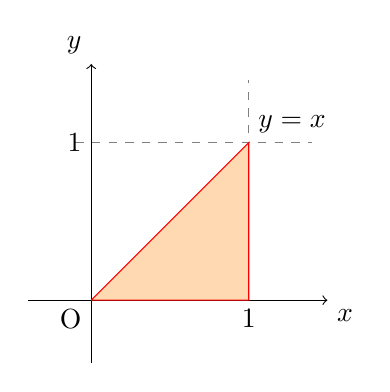
\begin{tikzpicture}[domain=0:1, yscale=2, xscale=2]
            
            \draw[very thin, dashed,color=gray] (-0.1,-0.1) grid (1.4,1.4);

            \draw[->] (-0.4,0) -- (1.5,0) node[below right] {$x$};
            \draw[->] (0,-0.4) -- (0,1.5) node[above left] {$y$};
            
            \draw (0,0) node[below left] {$\mathrm{O}$};
            \draw (1,0) node[below] {$1$};
            \draw (0,1) node[left] {$1$};
            \draw (1,1) node[above right] {$y=x$};

            \filldraw[color=red,fill=orange!30] (0,0) -- (1,1) -- (1,0) -- (0,0);

        \end{tikzpicture}
        \caption{領域$\Omega$}
        \label{fig:Omega}
    \end{figure}
    \begin{enumerate}[(i)]
        \item $x$で先に積分する,すなわち
        \begin{align}
            \int^1_0\qty(\int^1_y x(y-x)\dd{x})\dd{y}
        \end{align}
        の値は,
        \begin{align}
            \int^1_0\qty(\int^1_y x(y-x)\dd{x})\dd{y}
            &= \int^1_0\qty(\eval[-\frac{1}{3}x^3+\frac{1}{2}yx^2|_{x\coloneqq y}^{1})\dd{y}\\
            &= \int^1_0\qty(-\frac{1}{6}y^3+\frac{1}{2}y-\frac{1}{3})\dd{y}\\
            &= -\frac{1}{24}+\frac{1}{4}-\frac{1}{3}\\
            &= \frac{-1+6-8}{24}\\
            &= -\frac{1}{8}
        \end{align}
        である.
        \item $y$で先に積分する,すなわち
        \begin{align}
            \int^1_0\qty(\int^x_0 x(y-x)\dd{y})\dd{x}
        \end{align}
        の値は,
        \begin{align}
            \int^1_0\qty(\int^x_0 x(y-x)\dd{y})\dd{x}
            &= \int^1_0\qty(\eval[\frac{1}{2}xy-x^2y|_{y \coloneqq 0}^{x})\dd{x}\\
            &= \int^1_0\qty(-\frac{1}{2}x^3)\dd{x}\\
            &= -\frac{1}{8}
        \end{align}
        である.これらの値はFubiniの定理により一致することが確かめられる.
    \end{enumerate}
    \item 
    \begin{equation}
        B=\qty{ (x,y) \in \mathbb{R}^2 \where x^2+y^2\le 1 }
    \end{equation}
    である.
    \begin{align}
        B_1&=B \cap \qty{ (x,y) \in \mathbb{R}^2 \where x \ge 0, y \ge 0 } \\
        B_2&=B \cap \qty{ (x,y) \in \mathbb{R}^2 \where x \le 0, y \ge 0 } \\
        B_3&=B \cap \qty{ (x,y) \in \mathbb{R}^2 \where x \le 0, y \le 0 } \\
        B_4&=B \cap \qty{ (x,y) \in \mathbb{R}^2 \where x \ge 0, y \le 0 } 
    \end{align}
    とおくと,
    $B_i \cap B_j \quad(1\le i,j \le 4)$は直線なので面積は0.よって
    \begin{align}
        \iint_B \sqrt{1-x^2}\dd{x}\dd{y}
        &= \iint_{B_1} \sqrt{1-x^2}\dd{x}\dd{y} + \iint_{B_2} \sqrt{1-x^2}\dd{x}\dd{y} \\
        &+ \iint_{B_3} \sqrt{1-x^2}\dd{x}\dd{y} + \iint_{B_4} \sqrt{1-x^2}\dd{x}\dd{y} 
        \intertext{であり,$(x,y)\mapsto\sqrt{1-x^2}$は$x=0$と$y=0$に関して対称なので}
        \iint_B \sqrt{1-x^2}\dd{x}\dd{y}
        &=4\iint_{B_1} \sqrt{1-x^2}\dd{x}\dd{y}
    \end{align}
    である.

    この積分を求めるにあたって
    \begin{equation}
        \begin{cases}
            r&=\sqrt{x^2+y^2}\\
            \theta&=\mathrm{Arctan}\dfrac{y}{x}
        \end{cases}
    \end{equation}
    と変数変換すると,
    \begin{align}
        \mqty|\cos\theta & -r\sin\theta \\ \sin\theta & r\cos\theta|
        &=r\mqty|\cos\theta & -\sin\theta \\ \sin\theta & \cos\theta|\\
        &=r
    \end{align}
    であるので
    \begin{align}
        \iint_{B_1} \sqrt{1-x^2}\dd{x}\dd{y}
        &= \int^1_0 \int^{2\pi}_0 \sqrt{1-(r\cos\theta)^2}\ r \dd{r}\dd{\theta} \\
        &= \int^{2\pi}_0 \qty(\int^1_0 r\sqrt{1-\cos^2\theta r^2} \dd{r})\dd{\theta} \\
        &= \int^{2\pi}_0 \qty(\frac{1}{-3\cos^2\theta} \eval[(1-\cos^2\theta  r^2)^\frac{3}{2} |_{r\coloneqq 0}^{1})\dd{\theta} \\
        &= -\frac{1}{3} \int^{2\pi}_0 \frac{1}{\cos^2\theta} \qty(\sin^3\theta -1)\dd{\theta} \\
        &= -\frac{1}{3} \lim_{t\to \frac{\pi}{2}-0} \qty(\int^{t}_0 \frac{\sin^3\theta -1}{\cos^2\theta} \dd{\theta}) \\
        &= -\frac{1}{3} \lim_{t\to \frac{\pi}{2}-0} \qty(\int^{t}_0 (-\sin\theta) \qty(1-\frac{1}{\cos^2\theta}) \dd{\theta} - \int^{t}_0 \frac{1}{\cos^2\theta} \dd{\theta}) \\
        &= -\frac{1}{3} \lim_{t\to \frac{\pi}{2}-0} \qty( \cos t +\frac{1}{\cos t} - (1+\frac{1}{1}) - (\tan t - 0)) \\
        &= -\frac{1}{3} \lim_{t\to \frac{\pi}{2}-0} \qty( \cos t +\frac{1-\sin t}{\cos t} - 2) \\
        &= -\frac{1}{3}  \qty( -2 +\lim_{t\to \frac{\pi}{2}-0}\frac{\cos t}{1 + \sin t}) \\
        &= \frac{2}{3} 
    \end{align}
    である.よって
    \begin{align}
        \iint_B \sqrt{1-x^2}\dd{x}\dd{y}
        &=4\cdot \frac{2}{3}\\ 
        &=\frac{8}{3} 
    \end{align}
    である.
    \item 
    \begin{equation}
        I\coloneqq \int^1_0\qty(\int^1_{x^2}xe^{y^2}\dd{y})\dd{x}
    \end{equation}
    は,
    \begin{equation}
        D=\qty{(x,y)\in\mathbb{R}^2 \where x^2 \le y \le 1, 0\le x \le 1 }
    \end{equation}
    とすると,Fubiniの定理により
    \begin{align}
        \iint_D xe^{y^2} \dd{x}\dd{y}
        &=\int^1_0 \qty( \int^{\sqrt{y}}_0 xe^{y^2} \dd{x})\dd{y}
        \intertext{と一致するから,}
        I
        &=\int^1_0 \qty( \int^{\sqrt{y}}_0 xe^{y^2} \dd{x})\dd{y}\\
        &=\int^1_0 \qty( \eval[\frac{1}{2}x^2 e^{y^2} |_{x\coloneqq 0}^{\sqrt{y}})\dd{y}\\
        &=\frac{1}{2} \int^1_0  y e^{y^2} \dd{y}\\
        &=\frac{1}{2} \eval[\frac{1}{2} e^{y^2}|^1_{y\coloneqq 0} \dd{y}\\
        &=\frac{e-1}{4}
    \end{align}
    である.
\end{enumerate}

\end{document}